\documentclass[10pt,a4paper]{article}
\usepackage[utf8]{inputenc}
\usepackage[spanish]{babel}
\usepackage{a4wide}
\usepackage[sinEntregas]{caratula}
\usepackage{ulem}
\usepackage{marginnote}
\usepackage{fancyhdr}
\usepackage{lastpage}
\usepackage{float}
\usepackage{tikz}

\pagestyle{fancy}
\thispagestyle{fancy}
\addtolength{\headheight}{1pt}
\lhead{Bases de Datos}
\rhead{TP1}
\cfoot{\thepage /\pageref{LastPage}}
\renewcommand{\thesubsubsection}{\thesubsection.\alph{subsubsection}}

\title{Bases de Datos - TP 1}
\author{Bases de Datos, DC, UBA.}

\begin{document}

\fecha{8 de Mayo de 2015}

\materia{Bases de Datos}
%\submateria{Trabajo Pr\'actico Nº1}
\titulo{Trabajo Práctico Nº1}

\integrante{Allocati, Federico}{682/11}{fede.allocati@gmail.com}
\integrante{Izcovich, Sabrina}{550/11}{sizcovich@gmail.com}
\integrante{Pernigotti, Santiago}{870/11}{spernigotti@hotmail.com}
\integrante{Romano, Germán}{786/11}{romano.german@live.com.ar}

\maketitle

\tableofcontents

\newpage

\section{Introducción}

En el siguiente trabajo práctico, debimos diseñar e implementar una solución a un problema del mundo real utilizando herramientas de algún motor de base de datos relacional, en nuestro caso, \textit{SQLServer}.\\
\\
El problema a resolver consiste en la creación de un \textbf{Sistema de voto electrónico}. Para éste, debimos considerar que las votaciones se realizan en diferentes centros de votación que poseen mesas electorales compuestas por un presidente de mesa y su vicepresidente (o suplente). Por otro lado, pueden agregarse fiscales de cada partido político a la mesa que sirven para corroborar que el procedimiento se lleve correctamente a cabo.\\ Además, se agrega un técnico responsable de la máquina de votación, provista por el sistema. Por último, se agregan diferentes camionetas a los centros por si hay que cambiar o reparar alguna máquina. Para esto, se debe saber quién está asignado a cada una de ellas para lograr un control de las mismas.\\

El sistema debe asegurar lo siguiente:
\begin{itemize}
\item Se abarca todo el territorio de la nación y se soportan elecciones de cualquier cargo público de cada territorio que la compone. 
\item Se proveen los candidatos de cada elección y su partido político, como también la posibilidad de soportar varias elecciones desde el momento que se implemente.
\item Se soportan consultas populares hacia la ciudadanía.
\item Se respeta la confidencialidad de la elección del ciudadano.
\item Se guarda internamente el padrón electoral, esto es, en qué mesa vota cada ciudadano.
\item Se provee para cada mesa una máquina donde cada ciudadano puede elegir su opción.
\end{itemize}

Para lograr esto, debimos realizar un \textbf{Modelo de Entidad Relación} y su \textbf{Modelo Relacional} derivado. Luego, fue necesario diseñar la solución de forma física implementada en el motor de base de datos elegido. Por otro lado, realizamos el código correspondiente a las consultas/stored procedures/triggers pedidos. Finalmente, desarrollamos nuestros propios tests correspondientes a las funcionalidades de la API y extrajimos las conclusiones de la integralidad del trabajo práctico.

\newpage
\section{Modelo de Entidad Relación}

\begin{figure}[H] %[h] Aqui [b] para button [t] para top
\begin{center}
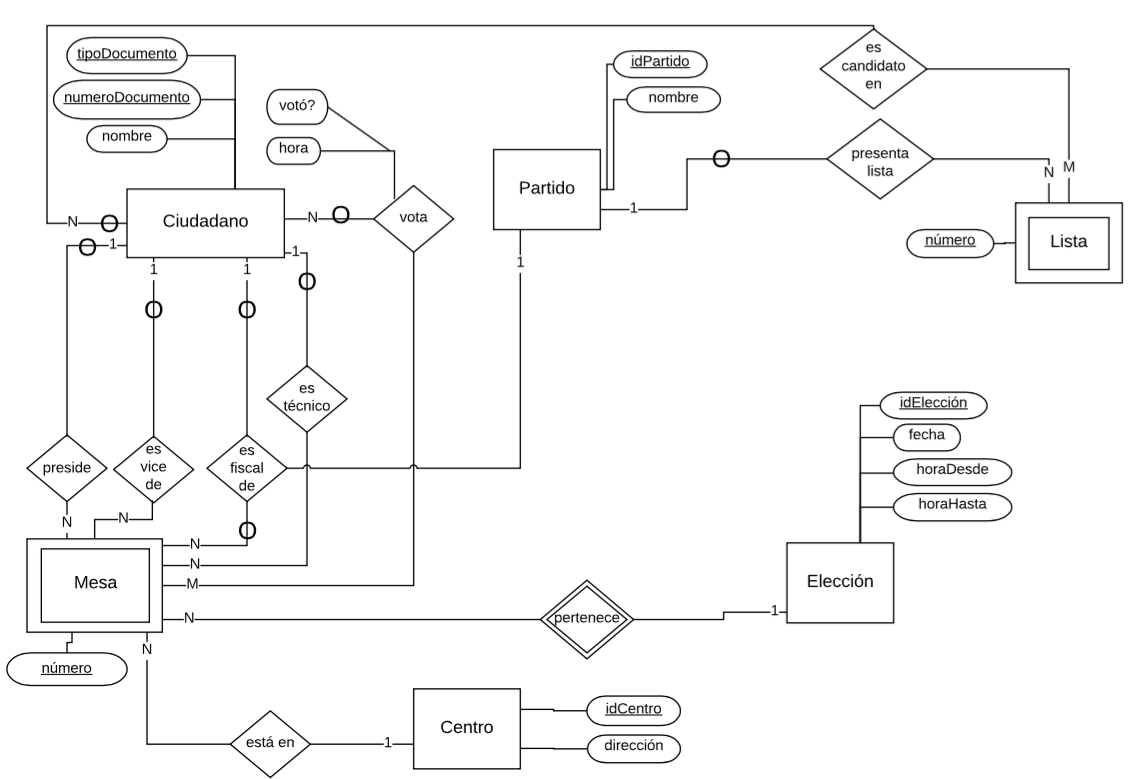
\includegraphics[width=470pt]{./diagramas/DER01.png}
\end{center}
\end{figure}

\begin{figure}[H] %[h] Aqui [b] para button [t] para top
\begin{center}
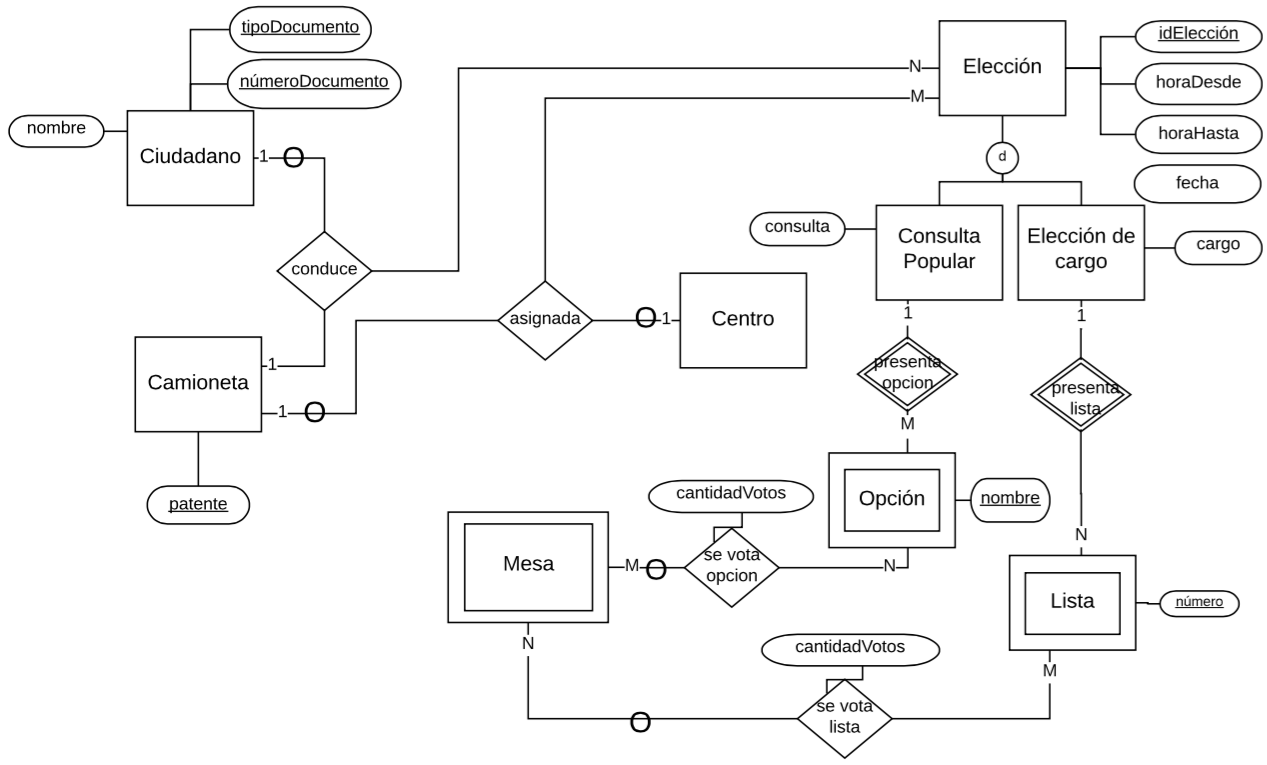
\includegraphics[width=470pt]{./diagramas/DER02.png}
\end{center}
\end{figure}

\subsection{Restricciones}
Presentamos las restricciones del Diagrama en lenguaje natural:
\begin{itemize}
\item Un ciudadano puede: presidir una mesa, o ser vicepresidente, o fiscal, o técnico, o chofer de camioneta, o ninguna de las anteriores. No puede desempeñar más de uno de los roles mencionados en una elección.
\item En una mesa se puede votar por una lista sólo si esa mesa pertenece a una elección de cargo.
\item En una mesa se puede votar por una opción (sí/no) sólo si esa mesa pertenece a una consulta popular.
\item Un ciudadano puede votar sólo en la mesa que le fue asignada en el padrón electoral.
\item Un candidato no puede figurar en dos listas distintas en una elección.
\item Un ciudadano no puede votar dos veces en una misma elección.
\item Un ciudadano puede presidir, vice-presidir, fiscalizar o ser el técnico encargado de hasta una mesa por elección.
\item Una camioneta puede estar asignada a un sólo centro.
\item En una mesa o bien se votan lista, o bien se votan opciones, según el tipo de elección en la que participe.
\item La camioneta que conduce un ciudadano para una elección debe estar asignada a esa misma elección.
\item Si un centro está asignado a una elección entonces ese centro tiene al menos una mesa que pertenece a esa elección.
\item La hora de votación de un ciudadano debe ser menor o igual a la hora de fin de la elección.
\item La hora de votación de un ciudadano debe ser mayor o igual a la hora de inicio de una elección.

\end{itemize}
\newpage
\section{Modelo Relacional}

\textbf{Elección}(\underline{idEleccion}, fecha, horaDesde, horaHasta, tipo)\\
PK = CK = \{idEleccion\}\\

\textbf{ConsultaPopular}(\underline{\underline{idEleccion}}, consulta)\\
PK = CK = FK = \{idEleccion\}\\

\textbf{ElecciónDeCargo}(\underline{\underline{idEleccion}}, cargo)\\
PK = CK = FK = \{idEleccion\}\\

\textbf{Opcion}(\underline{\underline{idEleccion}}, \underline{nombre})\\
PK = CK = \{(idEleccion, nombre)\}\\
FK = \{idEleccion\}\\

\textbf{Centro}(\underline{idCentro}, direccion)\\
PK = CK = \{idCentro\}\\

\textbf{Mesa}(\underline{\underline{idEleccion}}, \underline{numero}, \dashuline{idCentro}, \dashuline{(tipoDocumentoPresidente, numeroDocumentoPresidente)}, \dashuline{(tipoDocumentoVicepresidente, numeroDocumentoVicepresidente)}, \dashuline{(tipoDocumentoFiscal, numero
DocumentoFiscal)}, \dashuline{(tipoDocumentoTecnico, numeroDocumentoTecnico)})\\
PK = CK = \{(idEleccion, numero)\}\\
FK = \{idEleccion, idCentro, (tipoDocumentoPresidente, numeroDocumentoPresidente), (tipoDocumentoVicepresidente, numeroDocumentoVicepresidente), (tipoDocumentoTecnico, numeroDocumentoTecnico)\}\\

\textbf{Lista}(\underline{\underline{idEleccion}}, \underline{numero}, \dashuline{idPartido})\\
PK = CK = \{(idEleccion, numero)\}\\
FK = \{idEleccion, idPartido\}\\

\textbf{Partido}
(\underline{idPartido},nombre)\\
PK = CK = \{idEleccion\}\\

\textbf{SeVotaOpcion}
(\underline{\underline{idEleccion}}, \underline{\underline{numeroMesa}}, \underline{\underline{nombreOpcion}}, cantidadVotos)\\
PK = CK = \{(idEleccion, numeroMesa, nombreOpcion)\}\\
FK = \{(idEleccion, numeroMesa), (idEleccion, nombreOpcion)\}\\

\textbf{SeVotaLista}
(\underline{\underline{idEleccion}}, \underline{\underline{numeroMesa}}, \underline{\underline{numeroLista}}, cantidadVotos)\\
PK = CK = \{(idEleccion, numeroMesa, numeroLista)\}\\
FK = \{(idEleccion, numeroMesa), (idEleccion, numeroLista)\}\\

\textbf{Ciudadano}
(\underline{tipoDocumento}, \underline{numeroDocumento},nombre)\\
PK = CK = \{(tipoDocumento,numeroDocumento)\}\\

\textbf{Conduce}
(\underline{\underline{tipoDocumento}, \underline{numeroDocumento}, \underline{idEleccion}}, \dashuline{patente})\\
PK = \{(tipoDocumento, numeroDocumento, idEleccion)\}\\
CK = \{(tipoDocumento, numeroDocumento, idEleccion), (idEleccion, patente)\}\\
FK = \{(tipoDocumento, numeroDocumento), idEleccion, patente\}\\

\textbf{Asignada}
(\underline{\underline{idEleccion}, \underline{idCentro}}, \dashuline{patente})\\
PK = \{(idEleccion, idCentro)\}\\
CK = \{(idEleccion, idCentro), (idEleccion, patente)\}\\
FK = \{idEleccion, idCentro\}\\

\textbf{Camioneta}
(\underline{patente})\\
PK = CK = \{patente\}\\

\textbf{Vota}
(\underline{\underline{tipoDocumento}},\underline{numeroDocumento},\underline{\underline{idEleccion}, \underline{numeroMesa}}, votó?, hora)\\
PK = CK = \{(tipoDocumento, numeroDocumento, idEleccion, numeroMesa)\}\\
FK = \{(tipoDocumento, numeroDocumento), (idEleccion, numeroMesa)\}\\

\textbf{EsFiscalDe}
(\underline{\underline{tipoDocumento}, \underline{numeroDocumento},
\underline{idEleccion},
\underline{numeroMesa}}, \dashuline{idPartido})\\
PK = \{(tipoDocumento, numeroDocumento, idEleccion, numeroMesa)\}\\
CK = \{(tipoDocumento, numeroDocumento, idEleccion, numeroMesa),(idEleccion, numeroMesa, idPartido)\}\\
FK = \{(tipoDocumento, numeroDocumento), (idEleccion, numeroMesa), idPartido\}\\

\textbf{EsCandidatoEn}
(\underline{\underline{tipoDocumento}, \underline{numeroDocumento},
\underline{idEleccion},
\underline{numeroLista}})\\
PK = CK = \{(tipoDocumento, numeroDocumento, idEleccion, numeroLista)\}\\
FK = \{(tipoDocumento, numeroDocumento), (idEleccion, numeroLista)\}\\

\subsection{Restricciones Adicionales}
\begin{itemize}
\item \textit{ConsultaPopular.idEleccion} debe estar en \textit{Eleccion.idEleccion}

\item \textit{EleccionDeCargo.idEleccion} debe estar en \textit{Eleccion.idEleccion}

\item \textit{Eleccion.idEleccion} puede estar en \textit{EleccionDeCargo.idEleccion} o (exclusivo) \textit{ConsultaPopular.idEleccion} o (exclusivo) no estar en ninguno de los dos anteriores.

\item \textit{Partido.idPartido} puede no estar en \textit{Lista.idPartido}.

\item \textit{Lista.idPartido} debe estar en \textit{Partido.idPartido}.

\item \textit{SeVotaOpcion.nombreOpcion} debe estar en \textit{Opcion.nombre}.

\item \textit{SeVotaOpcion.numeroMesa} debe estar en \textit{Mesa.numero}.

\item \textit{SeVotaOpcion.idEleccion} debe estar en \textit{Opcion.idEleccion}.

\item \textit{Opcion.idEleccion} debe estar en \textit{ConsultaPopular.idEleccion}.

\item \textit{Opcion.nombre} debe estar en \textit{SeVotaOpcion.nombreOpcion}.

\item \textit{Opcion.idEleccion} debe estar en \textit{SeVotaOpcion.idEleccion}.

\item \textit{SeVotaLista.idEleccion} debe estar en \textit{EleccionDeCargo.idEleccion}.

\item \textit{SeVotaLista.numeroMesa} debe estar en \textit{Mesa.numero}.

\item \textit{SeVotaLista.numeroLista} debe estar en \textit{Lista.numero}.

\item \textit{Lista.numero} debe estar en \textit{SeVotaLista.numeroLista}.

\item \textit{Lista.idEleccion} debe estar en \textit{SeVotaLista.idEleccion}.

\item \textit{Mesa.numero} puede no estar en \textit{SeVotaLista.numeroLista}.

\item \textit{Mesa.numero} puede no estar en \textit{SeVotaLista.numeroMesa}.

\item \textit{Mesa.numero} puede no estar en \textit{SeVotaOpcion.numeroMesa}

\item \textit{Mesa.numero} debe estar en \textit{SeVotaOpcion.numeroMesa} o(exclusivo) en \textit{SeVotaLista.numeroMesa}

\item \textit{Lista.idEleccion} debe estar en \textit{EleccionDeCargo.idEleccion}.

\item \textit{ConsultaPopular.idEleccion} debe estar en \textit{Opcion.idEleccion}.

\item \textit{EleccionDeCargo.idEleccion} debe estar en \textit{Lista.idEleccion}.

\item \textit{Asignada.idCentro} debe estar en \textit{Centro.idCentro}.

\item \textit{Asignada.idEleccion} debe estar en \textit{Eleccion.idEleccion}.

\item \textit{Centro.idCentro} debe estar en \textit{asignada.idCentro}.

\item \textit{Eleccion.idEleccion} debe estar en \textit{asignada.idEleccion}.

\item \textit{Asignada.patente} debe estar en \textit{Camioneta.patente}.

\item \textit{Camioneta.patente} debe estar en \textit{Asignada.patente}.

\item \textit{Conduce.patente} debe estar en \textit{Camioneta.patente}.

\item \textit{Camioneta.patente} debe estar en \textit{Conduce.patente}.

\item \textit{Conduce.idEleccion} debe estar en \textit{Eleccion.idEleccion}.

\item \textit{Eleccion.idEleccion} debe estar en \textit{Conduce.idEleccion}.

\item \textit{(Ciudadano.tipoDocumento, Ciudadano.numeroDocumento)} puede no estar en \textit{(Conduce.tipoDocumento, Conduce.numeroDocumento)}.

\item \textit{(Conduce.tipoDocumento, Conduce.numeroDocumento)} debe estar en \textit{(Ciudadano.tipoDocumento, Ciudadano.numeroDocumento)}.

\item \textit{Lista.idPartido} debe estar en \textit{Partido.idPartido}.

\item \textit{Partido.idPartido} puede no estar en \textit{Lista.idPartido}.

\item \textit{EsCandidato.numero} debe estar en \textit{Lista.numero}.

\item \textit{Lista.numero} debe estar en \textit{EsCandidato.numero}.

\item \textit{(EsCandidato.tipoDocumento, EsCandidato.numeroDocumento)} debe estar en \textit{(Ciudadano.tipoDocumento, Ciudadano.numeroDocumento)}.

\item \textit{(Ciudadano.tipoDocumento, Ciudadano.numeroDocumento)} puede no estar en \textit{(EsCandidato.tipoDocumento, EsCandidato.numeroDocumento)}.

\end{itemize}
\newpage
\section{Supuestos asumidos}
Para un correcto diseño del Sistema, debimos tomar las siguientes decisiones sobre la situación presentada:
\begin{itemize}
\item Consideramos que los ciudadanos que están en el padrón se encuentran habilitados para votar.
\item Las elecciones no duran más de un día.
\item En una consulta popular, las únicas opciones para votar son Sí o No.
\item Una lista vale para una sola elección.
\end{itemize}
\newpage

\newpage
\section{Funcionalidades a implementar}

\textbf{Query:} \textit{Poder obtener los ganadores de las elecciones transcurridas en el último año.}\\

\textit{Stored Procedures:}

\begin{verbatim}
CREATE PROCEDURE GanadoresCargoUltimoAño
AS 
	SELECT todos.IdEleccion, todos.NumeroLista, todos.TotalVotos 
	FROM VotosPorListaPorEleccionDelAño() todos
	INNER JOIN
	(SELECT IdEleccion, max(TotalVotos) AS VotosGanador
	FROM VotosPorListaPorEleccionDelAño() 
	GROUP BY IdEleccion) ganador
	ON todos.IdEleccion = ganador.IdEleccion AND todos.TotalVotos = ganador.VotosGanador;
GO

CREATE PROCEDURE GanadoresOpcionUltimoAño
AS 
	SELECT todos.IdEleccion, todos.NombreOpcion, todos.TotalVotos 
	FROM VotosPorOpcionPorEleccionDelAño() todos
	INNER JOIN 
	(SELECT IdEleccion, max(TotalVotos) AS VotosGanador
	FROM VotosPorOpcionPorEleccionDelAño()
	GROUP BY IdEleccion) ganador
	ON todos.IdEleccion = ganador.IdEleccion AND todos.TotalVotos = ganador.VotosGanador;
GO
\end{verbatim}

\textit{Funciones:}

\begin{verbatim}
CREATE FUNCTION VotosPorOpcionPorEleccionDelAño()
RETURNS TABLE AS RETURN(
	SELECT v.IdEleccion, v.NombreOpcion, v.TotalVotos
	FROM VotosPorOpcionPorEleccion() v
	INNER JOIN Eleccion e ON e.IdEleccion = v.IdEleccion
	WHERE YEAR(e.Fecha) = YEAR(GETDATE()))
GO

CREATE FUNCTION VotosPorOpcionPorEleccion()
RETURNS TABLE AS RETURN(
	SELECT e.IdEleccion, s.NombreOpcion, sum(s.CantidadVotos) AS TotalVotos
	FROM Eleccion e 
	INNER JOIN SeVotaOpcion s ON e.IdEleccion = s.IdEleccion
	GROUP BY e.IdEleccion, s.NombreOpcion)
GO


CREATE FUNCTION VotosPorListaPorEleccionDelAño()
RETURNS TABLE AS RETURN(
	SELECT v.IdEleccion, v.NumeroLista, v.TotalVotos
	FROM VotosPorListaPorEleccion() v
	INNER JOIN Eleccion e ON e.IdEleccion = v.IdEleccion
	WHERE YEAR(e.Fecha) = YEAR(GETDATE()))
GO

CREATE FUNCTION VotosPorListaPorEleccion()
RETURNS TABLE AS RETURN(
	SELECT e.IdEleccion, s.NumeroLista, sum(s.CantidadVotos) AS TotalVotos
	FROM Eleccion e 
	INNER JOIN SeVotaLista s ON e.IdEleccion = s.IdEleccion	
	GROUP BY e.IdEleccion, s.NumeroLista)
GO
\end{verbatim}

\textbf{Query:} \textit{Poder consultar las cinco personas que más tarde fueron a votar antes de terminar la votación por cada centro electoral en una elección.}\\

\textit{Stored Procedures:}
\begin{verbatim}
CREATE PROCEDURE UltimosCincoEnVotarPorCentro
AS 
	SELECT IdEleccion, IdCentro, TipoDocumento, NumeroDocumento, Hora
	FROM 
	(SELECT v.IdEleccion, m.IdCentro, v.TipoDocumento, v.NumeroDocumento, v.Hora, RANK() 
	OVER(PARTITION BY m.IdEleccion, m.IdCentro ORDER BY m.IdEleccion, m.IdCentro, v.Hora 
	DESC) as Orden
	FROM Vota v INNER JOIN Mesa m ON v.numeroMesa = m.Numero AND v.IdEleccion = m.IdEleccion
	WHERE v.Voto = 1
	) t1
	WHERE Orden <= 5;
GO
\end{verbatim}

\textbf{Query:} \textit{Poder consultar quiénes fueron los partidos políticos que obtuvieron más del 20\% en las últimas cinco elecciones provinciales a gobernador.}\\

\textit{Stored Procedures:}
\begin{verbatim}
CREATE PROCEDURE PartidosConMasDel20EnLasUltimas5ParaGobernador
AS 
	SELECT TOP 5 e.IdEleccion, p.Nombre, v.TotalVotos
	FROM 
	(SELECT TOP 5 e.IdEleccion, e.Tipo, e.Fecha
	 FROM EleccionDeCargo ec
	 INNER JOIN Eleccion e ON e.IdEleccion = ec.IdEleccion
	 WHERE ec.Cargo = 'Gobernador'
	 ORDER BY Fecha DESC) e
	INNER JOIN VotosPorPartidoPorEleccion() v ON v.IdEleccion = e.IdEleccion
	INNER JOIN VeintePorCientoDeVotosPorEleccion() vp ON vp.IdEleccion = e.IdEleccion
	INNER JOIN Partido p ON p.IdPartido = v.IdPartido
	WHERE  v.TotalVotos > vp.VeintePorCientoDeVotos;
GO
\end{verbatim}

\textit{Funciones:}

\begin{verbatim}
CREATE FUNCTION VotosPorPartidoPorEleccion()
RETURNS TABLE AS RETURN(
	SELECT v.IdEleccion, l.IdPartido, sum(v.TotalVotos) AS TotalVotos
	FROM VotosPorListaPorEleccion() v
	INNER JOIN Lista l ON l.IdEleccion = v.IdEleccion AND l.Numero = v.NumeroLista
	GROUP BY v.IdEleccion, l.IdPartido)
GO

CREATE FUNCTION VotosPorListaPorEleccion()
RETURNS TABLE AS RETURN(
	SELECT e.IdEleccion, s.NumeroLista, sum(s.CantidadVotos) AS TotalVotos
	FROM Eleccion e 
	INNER JOIN SeVotaLista s ON e.IdEleccion = s.IdEleccion	
	GROUP BY e.IdEleccion, s.NumeroLista)
GO

CREATE FUNCTION VeintePorCientoDeVotosPorEleccion()
RETURNS TABLE AS RETURN(
	SELECT m.IdEleccion, (COUNT(*)*0.2) AS VeintePorCientoDeVotos
	FROM Mesa m 
	INNER JOIN Vota v ON m.IdEleccion = v.IdEleccion AND m.Numero = v.NumeroMesa
	WHERE v.Voto = 1
	GROUP BY m.IdEleccion
)
GO
\end{verbatim}
\newpage
\section{Conclusión}

El trabajo práctico consistió en diseñar y desarrollar una posible solución a un problema del mundo real. El mismo se basó en un sistema de voto electrónico capaz de abarcar todo el territorio de la nación y de soportar elecciones de cualquier cargo público.\\
En primer lugar, para lograr un diseño adecuado, debimos realizar un Modelo de Entidad Relación y su Modelo Relacional derivado.
Luego, debimos efectuar el diseño físico correspondiente implementado en el motor de base de datos \textit{SQLServer}.
Por otro lado, nos encargamos de implementar el código conveniente para las consultas/stored procedures/triggers pedidos.
Por último, realizamos los tests necesarios para evaluar las funcionalidades de la API.\\
A partir del trabajo realizado, podemos concluir que es indispensable un minucioso procedimiento de diseño y desarrollo para lograr una correcta solución a cualquier problema del mundo real. 
\end{document}